\begin{progprob}
    We can use a graph to represent rivalries between universities. Each
    node in the graph is a university, and an edge exists between two nodes
    if those two schools are rivals. For instance, the graph below represents
    the fact that OSU and Michigan are rivals, OSU and USC are rivals, UCB
    and USC are rivals, but UCSD does not have a rival.

    \begin{center}
    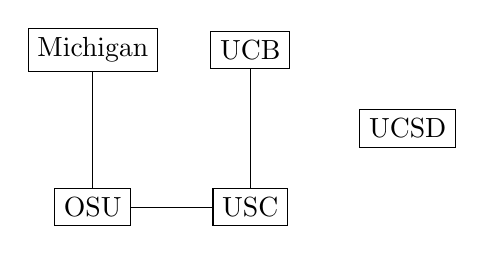
\begin{tikzpicture}
        \node[rectangle, draw] (osu) at (0,0) {OSU};
        \node[rectangle, draw] (um) at (0,2) {Michigan};
        \node[rectangle, draw] (usc) at (2,0) {USC};
        \node[rectangle, draw] (ucla) at (2,2) {UCB};
        \node[rectangle, draw] (ucsd) at (4,1) {UCSD};

        \draw (osu) -- (um);
        \draw (osu) -- (usc);
        \draw (ucla) -- (usc);

    \end{tikzpicture}
    \end{center}

    In a file called \python{assign_good_and_evil.py}, write a function
    \python{assign_good_and_evil(graph)} which determines if it is possible
    to label each university as either ``good'' or ``evil'' such that every
    rivalry is between a ``good'' school
    and an ``evil'' school. 
    The input to the function will be a graph of type \python{UndirectedGraph}
    from the \python{dsc40graph} package. If there is a way to label each node
    as ``good'' and ``evil'' so that every rivaly is between a ``good'' school
    and an ``evil'' school, your function should return it as a dictionary
    mapping each node to a string, \python{'good'} or \python{'evil'}; if such
    a labeling is not possible, your function should return \python{None}. 

    For example:
    \inputminted{python}{\thisdir/include/example.py}

    If in the above graph, there is also an edge between \python{'Michigan'} and \python{'USC'}, then there does not exist such a label and your funtcion should return \python{None}.

    Of course, there might be several ways to label the graph -- your code need only
    return one labeling.

    You can install \python{dsc40graph} by running 'pip install dsc40graph' in your terminal.

    \begin{soln}
        This can be solved using a graph search algorithm. We start by
        labeling the source node as either ``good'' or ``evil'' -- it doesn't
        matter which. We then label all of its neighbors with the opposite
        label. From there on, any time we visit a node and loop through the
        neighbors, we give each neighbor a label that is opposite the label
        of the node we are currently visiting.

        When looking through the neighbors, however, we may come across a
        node which already has already been assigned a label. If that label
        is the opposite of label of the node we are currently visiting, then
        all is fine. If the two labels are the same, then we have discovered
        that it is not possible to label the graph in this way.

        We will implement this idea by modifying the ``full'' BFS. We use
        the ``full'' version of the algorithm because the graph may not necessarily
        be connected (the example graph is not), yet we still wish to assign
        labels to every node. The code is shown below:

        \inputminted{python}{\thisdir/include-solution/assign_good_and_evil.py}

    \end{soln}
\end{progprob}
